\section{Геометрический смысл модуля и аргумента производной функции в
точке (рисунки и пояснения
обязательны).}\label{ux433ux435ux43eux43cux435ux442ux440ux438ux447ux435ux441ux43aux438ux439-ux441ux43cux44bux441ux43b-ux43cux43eux434ux443ux43bux44f-ux438-ux430ux440ux433ux443ux43cux435ux43dux442ux430-ux43fux440ux43eux438ux437ux432ux43eux434ux43dux43eux439-ux444ux443ux43dux43aux446ux438ux438-ux432-ux442ux43eux447ux43aux435-ux440ux438ux441ux443ux43dux43aux438-ux438-ux43fux43eux44fux441ux43dux435ux43dux438ux44f-ux43eux431ux44fux437ux430ux442ux435ux43bux44cux43dux44b.}

Пусть \(f'(z_0) \neq 0\).

\textbf{Определение:} Геометрический смысл модуля: \[
|\Delta w|=|f'(z_{0})|\cdot |\Delta z|\Leftrightarrow |\Delta w|=k\cdot |\Delta z|, k>0,
\] т.е. \(|f'(z_{0})|=k\) - коэффициент растяжения плоскости.
(гомотетия)

\textbf{Определение:} Геометрический смысл аргумента: \[
\Delta w=\underbrace{|f'(z_{0})|\cdot e^{ i\cdot \arg f'(z_{0}) }}_{f'(z_{0})}\cdot \Delta z
\] \(\Delta z\to e^{ i\cdot \arg f'(x_{0}) }\Delta z\) - поворот
\(\Delta z\) на угол \(\varphi=\arg f'(z_{0})\)

\textbf{Итого:} \(\Delta w\) есть композиция поворота на угол
\(\varphi\) \(+\) растяжение с коэффициентом \(|f'(z_{0})|\).

\pandocbounded{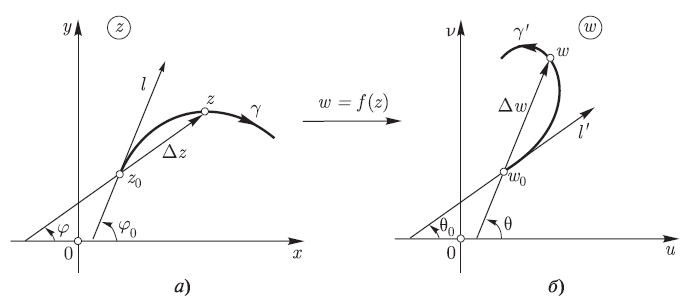
\includegraphics[keepaspectratio]{Вопросы/media/Pasted image 20260605234927.png}}

При отображении \(w = f(z)\) касательная \(l\) к кривой \(\gamma\) в
точке \(z_0\) переходит в касательную \(l'\) к образу \(\gamma'\) в
точке \(w_0 = f(z_0)\), повёрнутую на угол \(\arg f'(z_0)\). Здесь
\(\theta_{0}\) --- угол наклона \(l'\), \(\varphi_{0}\) --- угол наклона
\(l\) (на рисунке), откуда \(\arg f'(z_0) = \theta_{0} - \varphi_{0}\).
